\documentclass[a4paper]{article}
\usepackage[utf8]{inputenc}
\usepackage[polish]{babel}
\usepackage{polski}
%\usepackage{indentfirst}
%\usepackage{default}
%\usepackage{graphicx}
%\usepackage{inconsolata}
\usepackage{geometry}
\usepackage{graphicx}
\usepackage{array}
\usepackage{enumerate}
\usepackage{enumitem}
%\usepackage{parskip}
%\setlength{\parskip}{1ex}
\usepackage[T1]{fontenc}
\usepackage{color}
\definecolor{bluekeywords}{rgb}{0.13,0.13,1}
\definecolor{greencomments}{rgb}{0,0.5,0}
\definecolor{redstrings}{rgb}{0.9,0,0}

\begin{document}

\begin{titlepage}
    \begin{center}
        \bfseries
        \huge Politechnika Wrocławska
        \vskip.2in
        \textsc{\LARGE Wydział Elektroniki}
        \vskip.2in
        \Large Wizualizacja Danych Sensorycznych
        \vskip1.5in
        \emph{\huge Wizualizacja rozkładu ciśnienia cieczy na podstawie symulacji komputerowej}
    \end{center}

    \vskip1.4in

    \begin{minipage}{.50\textwidth}
        \begin{flushleft}
            \bfseries\large Prowadzący:\par \emph{Dr inż. Bogdan Kreczmer}
        \end{flushleft}
    \end{minipage}
    %\hskip.4\textwidth
    \begin{minipage}{.45\textwidth}
        \begin{flushright}
            \bfseries\large Studenci:\par \emph{ Adam Balawender \\ Krzysztof Kwieciński }
        \end{flushright}
    \end{minipage}

    \vskip1.3in

    \centering
    \bfseries
    \Large Semestr letni 2014/2015


\end{titlepage}

\section{Opis projektu}
Zgodnie z tematem projektu zajmiemy się komputerową symulacją zachowania cieczy oraz wizualizacją jej stanu i~rozkładu ciśnienia w zbiorniku z płynem.

Symulacja będzie obejmowała ruch cieczy w przekroju 2D wybranego naczynia. Ciecz zostanie przedstawiona na płaszczyźnie jako zbiór oddziaływujących ze sobą cząsteczek.
Postaramy się, żeby jej zachowanie było możliwie zbliżone do rzeczywistego.
Ruch płynu zostanie zamodelowany metodą numeryczną SPH (\textit{smoothed particle hydrodynamics - wygładzona hydrodynamika cząstek}).
Pozwoli to na realistyczne odwzorowanie zachowania cieczy.
Możliwe będzie badanie cieczy o różnych parametrach, dlatego też modelowane będą jej właściwości fizyczne: gęstość i~lepkość.
Dodatkowo mierzone będzie ciśnienie cieczy i zostanie ono zwizualizowane jako odcień koloru płynu.
Im będzie on ciemniejszy, tym wyższe ciśnienie będzie odzwierciedlał.

Najistotniejszymi funkcjonalnościami aplikacji będą:
\begin{itemize}
    \item symulacja zachowania cieczy w zależności od zadanych warunków początkowych,
    \item możliwość przedefiniowania parametrów cieczy (gęstości, lepkości),
    \item możliwość obserwacji wyniku symulacji (położenia cząsteczek i~rozkładu ciśnień).
\end{itemize}

\section{Plan pracy}
\subsection{Podział obowiązków}
Projekt zakłada powiązanie symulacji numerycznej (backend) z aplikacją prezentującą wyniki w formie graficznej (frontend). Za tę pierwszą odpowiedzialny będzie Adam
Balawender, za drugą Krzysztof Kwieciński. Obie części powinny mieć możliwość uruchomienia niezależnego, co ułatwi ich testowanie na wstępnych etapach oraz ich ocenę na końcowym etapie projektu.
\subsection{Harmonogram}
%\begin{enumerate}[label=Z\arabic*{.}]
\renewcommand{\arraystretch}{1.8}
\begin{tabular}{l || c | c }
Tydzień & Adam & Krzysztof                                                                                                                            \\\hline
    I    & \multicolumn{2}{ c }{ Opis projektu                                                                                                      } \\\hline
    II   & \multicolumn{2}{ c }{ Przegląd bibliotek Qt, szkic GUI                                                                                   } \\\hline
    III  & \multicolumn{2}{ c }{ Zapoznanie się z metodą SPH (Smoothed Particle Hydrodynamics)                                                      } \\\hline
    IV   & \multicolumn{2}{ c }{ Ustalenie struktur danych oraz API modułów                                                                         } \\\hline
    V    & \parbox[c]{6cm}{Implementacja klas zbiornika oraz cząsteczek cieczy }    & \parbox[c]{6cm}{Stworzenie statycznej wizualizacji zbiornika  } \\\hline
    VI   & \parbox[c]{6cm}{Implementacja metod uaktualniania położenia cząsteczek } & \parbox[c]{6cm}{Dodanie wizualizacji położenia cząstek cieczy } \\\hline
    VII  & \multicolumn{2}{ c }{ Analiza błędów działania programu                                                                                  } \\\hline
    VIII & \multicolumn{2}{ c }{ Skorygowanie działania programu                                                                                    } \\\hline
    IX   & Wyznaczanie ciśnienia w punkach zbiornika                       & Wizualizacja ciśnienia w punktach                                        \\\hline
    X    & \multicolumn{2}{ c }{ Weryfikacja projektu z założeniami                                                                                 } \\\hline
    XI   & \multicolumn{2}{ c }{ Odpowiednie modyfikacje programu                                                                                   } \\\hline
    XII  & \multicolumn{2}{ c }{ Napisanie raportu końcowego                                                                                        } \\
\end{tabular}
%\end{enumerate}


\subsection{Kamienie milowe}
\begin{enumerate}[label=K\arabic*{.}]
    \item Przeanalizowanie artykułów na temat SPH i zapoznanie się z tą metodą
    \item Zaimplementowanie struktur danych, modelu cieczy i relacji między cząsteczkami
    \item Wizualizacja symulowanego stanu cieczy
    \item Wizualizacja ciśnienia w poszczególnych punktach zbiornika
    \item Skończona dokumentacja
\end{enumerate}

\subsection{Diagram Gantta}
\begin{figure}[h] % rysunek pływający (początek) z deklaracją
    \begin{center}
        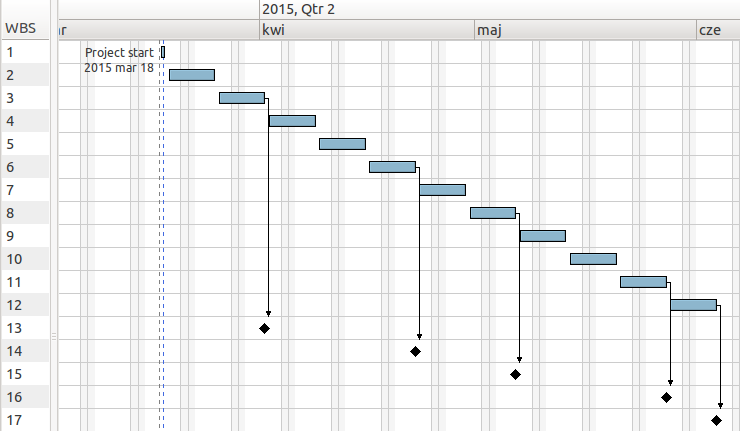
\includegraphics[width=\textwidth]{./rysunki/gantt.png}
    \end{center}
    \caption{Diagram Gantta}
    \label{fig:gantt}
\end{figure}

\section{Notatka dla Prowadzącego}
Szanowny Panie Doktorze,
Przypominamy, że na drodze wyjątku zgodził się Pan przyjąć opis naszego projektu wzbogacony o podział harmonogramu między członków grupy z pominięciem kary za spóźnienie.
\end{document}
